\section{Client-server architecture}

In the client-server architecture, hardware components include a server responsible for data management and a client focused on presentation layout.
\begin{figure}[H]
    \centering
    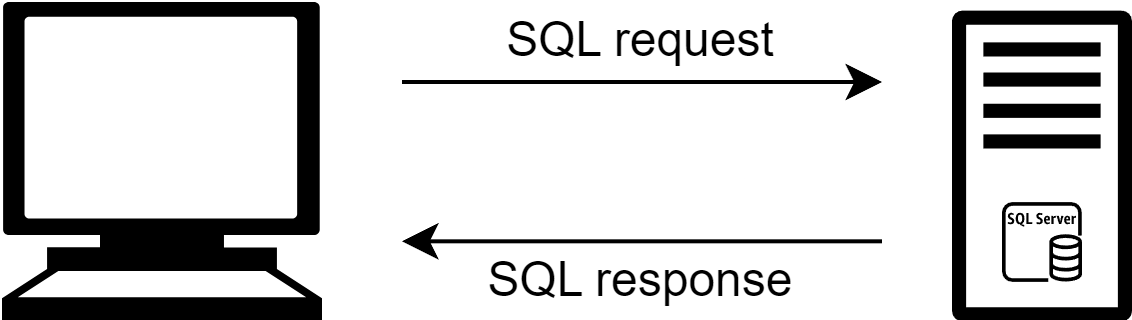
\includegraphics[width=0.4\linewidth]{images/cs.png}
\end{figure}
The client software issues requests to the server via SQL queries and handles both business logic and presentation logic. 
The server software processes these queries and sends the resulting data back to the client, focusing on data management.

The network topology is typically organized as a Local Area Network (LAN) with one or more servers and multiple clients.